\chapter{When a Loan Becomes a Business You Never Wanted}

The interview begins with a blunt question: what was the worst financial decision? The answer is equally blunt, and it comes before the story: getting involved in something one does not want to be involved in. The case is a construction loan that was supposed to be temporary and collateralized, but the real exposure widened into management failure, years of operating work, a tragic accident, the loss of the company, and a reported personal loss close to \(\$3{,}000{,}000\). These notes treat the interview as a compact lesson in entrepreneurial exposure: not a formula for pricing debt, but a method for seeing when a financial instrument can become an unwanted operating obligation. The source is the School of Hard Knocks interview, curated by LazyingArt LLC through Video2Book.

\section{The Question and the Rule}

The speaker is asked for the worst financial decision he has made over his life. He does not begin with the size of the loss. He does not begin with the industry. He begins with the form of the mistake:

\begin{equation}
\text{bad involvement}
=
\text{entering a problem one does not want to own}.
\end{equation}

This is a reconstruction of the logic, not a board equation. The spoken answer is simpler: the mistake was getting involved in things he did not want to be involved in. The order matters. The rule appears first. The story then supplies the mechanism.

We should not flatten the rule into a vague slogan. In the transcript, the unwanted involvement is specific: a construction loan connected to a business he really did not want to be in. The issue is therefore not only that capital was lost. The issue is that the transaction carried a possible future role he already knew he did not want.

\section{A Loan That Looked Bounded}

The concrete case begins as financing. The speaker describes doing a construction loan on a business he did not want to enter. He adds that he was talked into it by a friend, so the decision already sits between two forces: internal reluctance and social persuasion.

Then comes the line that makes the case analytically interesting. The loan was supposed to be temporary, and everything was collateralized. Those words are meant to make risk look bounded. Temporary means the exposure should end. Collateralized means there is supposed to be property or security behind the debt.

If we looked only at the stated deal form, we might summarize the exposure as

\begin{equation}
E_{\text{nominal}}
=
E_{\text{capital under loan terms}}.
\end{equation}

Here \(E_{\text{nominal}}\) is the risk one sees by reading the transaction as a loan and nothing more. The lecture's movement is the discovery that this was an incomplete description. The nominal exposure was not the lived exposure.

\subsection{Question \& Answer}

\paragraph{Question.}
If the construction loan was temporary and collateralized, why could it still become the speaker's worst financial decision?

\paragraph{Answer.}
Because the financial description did not exhaust the entrepreneurial exposure. Collateral can reduce one form of capital risk, and a temporary term can reduce one form of duration risk, but neither prevents management failure. Once management fails, the lender may face a new question: either watch the business deteriorate, or step into a business he never wanted to operate.

The distinction is

\begin{equation}
\text{nominal loan risk}
\neq
\text{total entrepreneurial exposure}.
\end{equation}

That is the central turn in the story. The loan looked bounded at the level of the instrument. It became unbounded at the level of responsibility.

\begin{table}
\centering
\begin{tabular}{p{0.27\linewidth} p{0.31\linewidth} p{0.29\linewidth}}
\hline
Stated protection & Exposure not removed & Transcript outcome \\
\hline
Temporary loan & Time cost if the business fails & A couple of years spent turning it around \\
Collateralized deal & Operating responsibility beyond paper security & Management was failing \\
Passive financing role & Severe business event risk & Accident, death, company loss \\
\hline
\end{tabular}
\end{table}

\section{The Exposure Update}

Now the story turns. The company ended up with failing management. The speaker says he had to step in and spend a couple of years turning it around. This is the important mutation. The nominal role is lender. The practical role becomes operator.

A cautious decomposition of total exposure is

\begin{align}
E_{\text{total}}
&=
E_{\text{capital}}
+
E_{\text{time}}
+
E_{\text{operating}}
+
E_{\text{tail}}.
\end{align}

This notation is a note-writing device, not a transcript quotation. It helps us keep the categories distinct. \(E_{\text{capital}}\) is the money at risk. \(E_{\text{time}}\) is the cost of years spent inside the problem. \(E_{\text{operating}}\) is the responsibility created by failed management. \(E_{\text{tail}}\) is exposure to severe events attached to the business itself.

The update is the useful part:

\begin{align}
E_{\text{total}}^{(0)}
&=
E_{\text{capital}},
\\
E_{\text{total}}^{(1)}
&=
E_{\text{capital}}
+
E_{\text{operating}},
\\
E_{\text{total}}^{(2)}
&=
E_{\text{capital}}
+
E_{\text{operating}}
+
E_{\text{time}},
\\
E_{\text{total}}^{(3)}
&=
E_{\text{capital}}
+
E_{\text{operating}}
+
E_{\text{time}}
+
E_{\text{tail}}.
\end{align}

At the beginning, the deal could be imagined as capital exposure. When management failed, operating exposure entered. When he spent a couple of years turning the company around, time exposure entered. When the tragic accident occurred, tail exposure entered. The story is not that these quantities were known precisely in advance. The story is that they were possible, and the speaker already knew he did not want the underlying business.

\begin{figure}
\centering
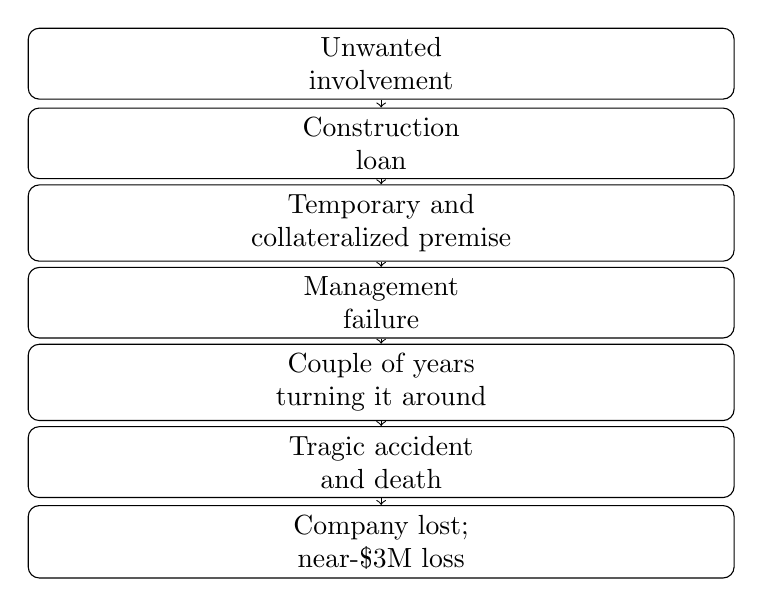
\begin{tikzpicture}[scale=0.92]
\node[draw, rounded corners, align=center, text width=0.72\linewidth] (a) at (0,0) {Unwanted\\involvement};
\node[draw, rounded corners, align=center, text width=0.72\linewidth] (b) at (0,-1.10) {Construction\\loan};
\node[draw, rounded corners, align=center, text width=0.72\linewidth] (c) at (0,-2.20) {Temporary and\\collateralized premise};
\node[draw, rounded corners, align=center, text width=0.72\linewidth] (d) at (0,-3.30) {Management\\failure};
\node[draw, rounded corners, align=center, text width=0.72\linewidth] (e) at (0,-4.40) {Couple of years\\turning it around};
\node[draw, rounded corners, align=center, text width=0.72\linewidth] (f) at (0,-5.50) {Tragic accident\\and death};
\node[draw, rounded corners, align=center, text width=0.72\linewidth] (g) at (0,-6.60) {Company lost;\\near-\$3M loss};

\draw[->] (a) -- (b);
\draw[->] (b) -- (c);
\draw[->] (c) -- (d);
\draw[->] (d) -- (e);
\draw[->] (e) -- (f);
\draw[->] (f) -- (g);
\end{tikzpicture}
\end{figure}

The diagram is a reconstruction from the transcript. It is intentionally vertical and narrow: the point is not to make a dense financial model, but to preserve the order in which the exposure widened.

\section{The Tail Event and the Number}

After the turnaround work, the story does not become a recovery story. The speaker says that a tragic accident occurred and that somebody unfortunately passed away. He then states the business consequence: it ended up costing the entire company.

This is where we need discipline. The transcript does not give the legal structure, the insurance position, the collateral value, the loan amount, the ownership percentage, or the precise causal mechanics. The source gives us the sober sequence: accident, death, company loss, and a personal loss close to three million dollars.

The one hard quantitative anchor is therefore

\begin{equation}
L \approx \text{\$}3{,}000{,}000,
\end{equation}

where \(L\) denotes the speaker's reported personal loss. It is not a reconstructed balance sheet.

Putting the story into one causal line, we have

\begin{equation}
\begin{aligned}
\text{reluctance}
&\to
\text{construction loan}
\to
\text{management failure} \\
&\to
\text{turnaround work}
\to
\text{tragic event} \\
&\to
\text{company loss}
\to
L \approx \text{\$}3{,}000{,}000.
\end{aligned}
\end{equation}

This is why the initial reluctance was not noise. It was information. The speaker's unwillingness to be in the business was relevant because the downside of the loan included being pulled into that business.

\section{The Decision Rule}

The closing movement returns to the opening rule. The speaker says the experience taught him not to get involved in something he does not want to get involved in. He also says his gut instinct was telling him from day one not to do it, but he did it anyway.

A disciplined version of that rule is not merely ``trust your gut.'' It is a screen for unwanted ownership:

\begin{equation}
\text{Reject the deal if}
\qquad
E_{\text{total}} > W_{\text{own}}.
\end{equation}

Here \(W_{\text{own}}\) means the willingness to own the problem if the deal stops behaving according to its optimistic description. This is not a pricing equation. It is a refusal equation. It asks whether we would still want the situation if the protective story failed.

For this interview, the answer was already present at the beginning. He did not want to be in the business. The later events revealed the cost of overriding that signal. A temporary, collateralized loan may reduce some financial risk, but it does not necessarily remove the possibility of becoming responsible for a business, crisis, or operating role.

\section{Summary}

The interview gives a compact theory of entrepreneurial exposure. A deal can be bounded on paper and unbounded in practice. The speaker entered a construction loan on a business he did not want to be in, after being talked into it by a friend. The loan was supposed to be temporary and collateralized. Management failed, he spent a couple of years turning the company around, a tragic accident followed, the company was lost, and he reports losing close to \(\$3{,}000{,}000\).

The durable lesson is not that every collateralized loan is dangerous. It is narrower and sharper: before accepting a transaction, ask what role the downside could force us to occupy. If the answer is a business, crisis, or responsibility we already know we do not want, then the real exposure is larger than the loan.
